% % % % % % % % % % % % % % 
% 
% Skript zu NUMERIK I
% WS14/15
% von Prof. Dr. Blank
% Universität Regensburg
% 
% 
%	Kap. 6: Interpolation
% 
% % % % % % % % % % % % % % 


\chapter{Interpolation}

Es seien diskrete Werte $f_i=f(t_i)$ und 
eventuell $f_i^{(j)} = f^{(j)}(t_i)$ 
an den Punkten $t_i$ gegeben (z.B. Messdaten).\\
Gesucht ist nun eine zugehörige Funktion $\varphi$.

Anwendungsfeld solcher Probleme ist z.B. CAD (computer aided
design).

Eine naheliegende Forderung ist die
\textbf{Interpolationseigenschaft}\index{Interpolation!-eigenschaft}
\begin{gather*}
  \varphi^{(j)} (t_i) = f_i^{(j)}\qquad \text{gegeben für alle } i,j ,
\end{gather*}
d.h. $\varphi$ und $f$ sollen an den \textbf{Knoten} oder 
\textbf{Stützstellen}\index{Stützstelle} $t_i$ übereinstimmen.
Die $f_i^{(j)}$ heißen Stützwerte\index{Stützwert}.
\imagemissing{Verschiedene Grafen zu Stützstellen-Stützwert-Paaren}\label{im6.1}
$\varphi$ soll zusätzlich meist leicht an einer beliebigen Stelle $t$
auswertbar sein. \\
Es bietet sich z.B. an 
\begin{itemize}
\item Polynome: $\varphi(t) = a_0+\dots +a_n t^n$
\item rationale Funktion: $\varphi(t) = \frac{p(t)}{q(t)} $\\
  (insbesondere, falls Pole vorliegen)
\item Spline, d.h. stückweise Polynome
\item trigonometrische Funktionen, Fouriertransformationen:\\
  $ \varphi (t) = \sum_{j=1}^{\infty} a_je^{-2\pi ijt}$\\
  (insbesondere für periodische Funktionen)
\end{itemize}

\sectione{Polynom-Iterpolation}
Wir definieren als 
\begin{gather}
  \p_n \coloneqq \left\{ p \in \R[x]\,\middle\vert\,
    p= \sum_{i=0}^{n} a_ix^i \text{ mit } a_i\in\R \right\}
  \label{VI.1.1}
\end{gather}
den Raum aller Polynome\index{Polynomraum} mit $deg(p)\leq n$.\\
Die Monome $1,x, \dots , x^n$ bilden eine Basis von $\p_n$
und es gilt $dim\p_n = n+1$.

\extrasection{a)}{Lagrangesche Interpolationsformel und Lemma von Aitken}

% \subsectione{Satz}
\begin{Satze}\label{6.1.1}
  Zu beliebigen $n+1$ Stützpunkten $(x_i, f_i)_{i=0, \dots n}$ 
  mit $x_i\neq x_k$ für $i\neq k$,
  gibt es genau ein $p\in \p$ mit $p(x_i) = f_i$ für $i=0,
  \dots ,n$.\\
  $p$ heißt \textbf{Interpolationspolynom}\index{Interpolation!-polynom}
  und wird mit $p(f|x_0, \dots, x_n) $ bezeichnet.
\end{Satze}

\begin{proof}~
  \begin{enumerate}[a)]
  \item \textit{Eindeutigkeit}:
    Seien $p_1, p_2\in \p_n$ mit $p_1(x_i)=p_2(x_i) = f_i$
    für $i=0, \dots, n$.
    Dann ist $p\coloneqq p_1-p_2 \in\p_n$
    mit mindestens $n+1$ Nullstellen. \\
    Daraus folgt bereits, dass $p\equiv 0$, also $p_1\equiv p_2$.

  \item \textit{Existenz}: 
    Betrachte die Polynome $L_i\in\p_n$ für $i=0, \dots, n$
    mit 
    \begin{gather}
      L_i(x_k) = \delta_{ik}\quad \text{für } i,k=0, \dots, n 
      \label{VI.1.2}
    \end{gather}
    Diese sind gegeben durch
    \begin{gather}
      L_i(x) \coloneqq \frac{(x-x_0)\cdot \dotsc
        \cdot (x-x_{i-1})(x-x_{i+i}) \cdot \dotsc
        \cdot (x-x_n)}
      {(x_i-x_0)\cdot \dots
        \cdot (x_i-x_{i-1})(x_i-x_{i+i}) \cdot \dotsc
        \cdot (x_i-x_n)}
      \label{VI.1.3}
    \end{gather}
    und sind nach a) eindeutig. \\
    Sie heißen \textbf{Lagrange-Polynome}\index{Lagrange-Polynome}.
  \end{enumerate}
  Die \textbf{Lagrange-Interpolationsformel}\index{Interpolation!Lagrange-Formel}
  \begin{gather}
    p(x) = \sum_{i=0}^{n} f_iL_i(x)
    \label{VI.1.4}
  \end{gather}
  bestimmt somit $p(f\mid x_0, \dots, x_n)$,
  da $p\in\p_n$ und $p(x_i) = f_i$ für $i=0,\dots, n$.
\end{proof}

Mit \eqref{VI.1.4} folgt weiterhin
\begin{enumerate}[a)]
\item $p$ hängt linear von den Stützwerten $f_i$ ab.
\item Die Lagrange-Polynome bilden eine Basis des $\p_n$.
\end{enumerate}

Die Lagrange-Interpolationsformel ist,
wenn auch für theoretische Fragen günstig,
für praktische Zwecke zu rechenaufwändig.

Zur Auswertung des Interpolationspolynoms $p(f\mid x_0,\dots, x_n)$
an einer festen Stelle $\overline{x}$, d.h.
um den Wert $p(\overline{x} ) $ zu berechnen,
benötigt man:

% \subsectione{Lemma von Aitken}
\begin{Leme}[Lemma von Aitken]\index{Lemma von Aitken}
  Für das Interpolationspolynom $p(f\mid x_0, \dots, x_n)$ gilt die 
  Rekursionsformel
  \begin{gather}
    p(f\mid x_0, \dots, x_n) (x) = \frac{(x_0-x)p(f\mid x_1,\dots, x_n)(x) -
      (x_n-x)p(f\mid x_0,\dots, x_{n-1})(x)}
    {(x_0-x_n)}
    \label{VI.1.5}
  \end{gather}
  für $n>0$.	
\end{Leme}

\begin{proof}
  Sei die rechte Seite von \eqref{VI.1.5} definiert als $\varphi(x)$.
  Dann ist $\varphi\in\p_n$ und 
  \begin{alignat*}{3}
    \varphi(x_i) &= \frac{(x_0-x_i)f_i-(x_n-x_i)f_i}{x_0-x_n}= f_i\quad
    &&&\text{für } i&=1,\dots , n-1\\
    \varphi(x_0) &= \frac{0-(x_n-x_0)f_0}{x_0-x_n} = f_0
    &&&\text{für } i&=0\\
    \varphi(x_n) &= \frac{(x_0-x_n)f_n-0}{x_0-x_n} = f_n
    &&&\text{für } i&=n\\
  \end{alignat*}
  Damit ist $p(f\mid x_0, \dots, x_n) = \varphi$ aufgrund der Eindeutigkeit.
\end{proof}


% -----------------------------------------------------------------------

Weiterhin gilt
\marginpar{03.12.2014}
\begin{gather}
  p(f\mid  x_i)(x) = f_i\quad \forall x\in\R
  \label{VI.1.6}
\end{gather}
Definiere nun für ein festes $\overline{x}$
\begin{gather}
  P_{ik} \coloneqq p(f\mid  x_{i-k}, \dots, x_{i})(\overline{x})
  \label{VI.1.7}
\end{gather}
Dann lässt sich der Wert
\begin{gather*}
  p(\overline{x}) = p(f\mid  x_0, \dots , x_n)(\overline{x})= P_{nn}
\end{gather*}
nach \eqref{VI.1.5} wie folgt berechnen:


\subsectione{Schema von Neville}
\index{Neville-Schema}
Setze $P_{i0} = f_i$ für $i=0, \dots , n$ und
\begin{gather}
  P_{ik} = P_{i,k-1}+\frac{\overline{x}-x_i}{x_i-x_{i-k}}
  \cdot \left( P_{i,k-1}-P_{i-1,k-1}\right)
  \quad \text{für } 1\leq k\leq i\leq n
  \label{VI.1.8}
\end{gather}
\begin{gather*}
  \begin{array}{r|cccccccccc}
    x_i\backslash k & 0 && 1 && \dots \\
    \cline{1-8}
    x_0 & f_0 & \searrow\\
    x_1 & f_1 & \rightarrow & P_{11}&\searrow\\
    \vdots & \vdots && P_{21} &\rightarrow& P_{22} \\
    \vdots  & \vdots && && &\ddots \\
    x_n & f_n && P_{n1} && \dots &&  P_{nn}
  \end{array}
\end{gather*}
\eqref{VI.1.8} benötigt weniger Multiplikationen als 
\eqref{VI.1.5} und ist deutlich billiger als
\eqref{VI.1.4}.
Pro Auswertung an einer Stelle $\overline{x}$ sind
$\frac{n(n+1)}{2}$ Multiplikationen und Divisionen notwendig.\\
Soll das Interpolationspolynom an mehreren Stellen ausgewertet werden,
ist das Schema von Neville zu teuer.

\extrasection{b)}{Newtonsche Interpolationsformel}
Betrachte folgende Basisdarstellung eines Polynoms $p\in\p_n$
\begin{align}
  p(x) = \sum_{i=0}^{n}a_i \prod_{j=0}^{i-1} (x-x_j)
  \label{VI.1.9}
\end{align} 
Damit wird $p$ zu 
\begin{gather}
  p(x)= \Bigg(\dots \bigg(\Big(
  \big(a_n(x-x_{n-1})+a_{n-1}\big)\cdot(x-x_{n-2})+a_{n-2}\Big)
  \cdot (x-x_{n-3})+a_{n-3}\bigg) \dots\dots\Bigg)
  \label{VI.1.10}
\end{gather}
Es ergibt sich für bekannte $a_i\in\R$:

\subsectione{Das Horner-Schema zur Auswertung p(x)}
\index{Horner-Schema}
\begin{pseudocode}{6cm}
  $p=a_n$ \\
  \textbf{for} $k=n-1:-1:0$\\
  |\>  $p=p(x-x_k)+a_k$\\
  \textbf{end}
\end{pseudocode}

Pro Auswertung benötigt es $n$ Multiplikationen.\\
Zur Bestimmung der notwendigen Koeffizienten $a_0, \dots, a_n$
von $p(f\mid  x_0, \dots , x_n)$ kann folgende 
Vorwärtssubstitution verwendet werden
\begin{align*}
  f_0 &= p(x_0) = a_0\\
  f_1 &= p(x_1) = a_0+a_1(x_1-x_0)\\
      &\vdots\\
  f_n &=p(x_n) = a_0 + \dots + a_n(x_n-x_0)\cdot\dots\cdot(x_n-x_{n-1})
\end{align*}
Es geht jedoch noch billiger, wie gleich zu sehen ist.

\begin{Defe}~
  \begin{enumerate}[a)]
  \item Die folgenden Polynome heißen \textbf{Newton-Polynome}
    \index{Newton-Polynome}
    \begin{align*}
      w_0(x) &\coloneqq 1\\
      w_i(x) &\coloneqq \prod_{j=0}^{i-1} (x-x_j)
             &\text{für } i\geq 1
    \end{align*}
  \item Die $n$-te dividierte Differenz $[x_0,\dots , x_n]f$
    \index{dividierte Differenzen}
    ist definiert durch
    \begin{align}\nonumber
      [x_i]f &\coloneqq f_i\\
      [x_i,\dots, x_n]f 
             &\coloneqq
               \frac{[x_{i+1},\dots,x_n]f-[x_i,\dots,x_{n-1}]f}
               {x_n-x_i}
               \label{VI.1.11}
    \end{align}
    für $x_n\neq x_i$.
  \end{enumerate}
\end{Defe}


\begin{Satze}\label{6.1.6}
  Sei $p(f\mid  x_0,\dots ,x_n)(x)=\sum_{i=0}^{n}a_iw_i(x) = 
  a_nx^n+ \sum_{i=0}^{n-1}c_ix^i$, dann gilt
  \begin{gather*}
    a_n= [x_0, \dots, x_n]f
  \end{gather*}
  und für jede Permutation $\sigma \in S_n$
  \begin{gather*}
    [x_0,\dots, x_n]f= [x_{\sigma(0)},\dots , x_{\sigma(n)}]f
  \end{gather*}
  Somit ist $[x_0, \dots, x_n]f$ wie p unabhängig von der
  Reihenfolge der Knoten und es gilt für $x_l\neq x_j$
  \begin{gather}
    [x_i, \dots, x_k] f= \frac{[x_i,\dots,\widehat{x}_j,\dots,x_k]f
      -[x_i,\dots,\widehat{x}_l,\dots,x_k]f}
    {x_l-x_j}
    \label{VI.1.12}
  \end{gather}
  wobei $\widehat{\bullet}$ bedeutet, dass dieser Knoten
  weggelassen wird.
\end{Satze}

\begin{proof}
  Wir zeigen den Satz per Induktion.\\
  Induktionsanfang mit $n=0$:
  \begin{gather*}
    p(f\mid x_0) (x) = f_0 = a_0 = [x_0]f
  \end{gather*}
  Induktionsschritt $n \rightarrow n+1$:
  Nach dem Lemma von Aitken gilt \eqref{VI.1.5}, also 
  \begin{gather*}
    p(f\mid x_0, \dots, x_{n+1}) (x) 
    = \frac{(x_0-{\boldsymbol x}){\boldsymbol p}(f\mid x_1,\dots, x_{n+1})(x) -
      (x_{n+1}-{\boldsymbol x}){\boldsymbol p}(f\mid x_0,\dots, x_{n})(x)}
    {(x_0-x_{n+1})}
  \end{gather*}
  Nach Induktionsvoraussetzung gilt also 
  für den Koeffizienten zu  $x^{n+1}$, welcher $a_{n+1}$ ist,
  \begin{align*}
    a_{n+1} &= \frac{-[x_1,\dots, x_{n+1}]f+[x_0,\dots,x_n]f}
              {x_0-x_{n+1}}\\
            & = [x_0, \dots , x_{n+1}] f
  \end{align*}
\end{proof}


\begin{Satze}[Newtonsche Darstellung]\label{6.1.7}
  \index{Polynomraum!Newtonsche Darstellung}
  Es gilt 
  \begin{gather}
    p(f\mid  x_0, \dots , x_n)(x) 
    = \sum_{i=0}^{n}[x_0,\dots, x_i]f\cdot w_i(x)
    \label{VI.1.13}
  \end{gather}
  und $\left\{w_k\middle\vert k\in \{0,\dots,n\}\right\}$
  bildet Basis von $\p_n$.
\end{Satze}

\begin{proof}
  Wir zeigen \eqref{VI.1.10} per Induktion.\\
  $n=0$ ist klar.\\
  $n-1\rightarrow n$: Sei $p_n(x)\coloneqq p(f\mid  x_0,\dots,x_n)(x)
  = [x_0,\dots, x_n]f \cdot w_n(x) + q_{n-1}(x)$ mit
  $q_{n-1}\in\p_{n-1}$ und $q_{n-1}(x_i)=p_{n-1}(x_i)=f_i$
  für $i=0,\dots ,n-1$, da $w_n(x_i)=0$.\\
  Damit folgt
  \begin{gather*}
    q_{n-1} = p(f\mid x_0, \dots, x_{n-1})
    =\sum_{i=0}^{n-1}[x_0,\dots, x_i]f\cdot w_i(x)
  \end{gather*}
  nach Induktionsvoraussetzung. 
  Es folgt Gleichung  \eqref{VI.1.13}.\\
  $\left\{w_0, \dots,w_n\right\}$ sind linear unabhängig
  und jedes Polynom $\varphi\in\p_n$
  lässt sich wegen $q(x)=p(q\mid x_0,\dots,x_n)(x)$
  durch \eqref{VI.1.13} darstellen.
\end{proof}

Entsprechend zum Schema von Neville für $p(\overline{x})$
ergibt sich zur Berechnung der Koeffizienten $a_i=[x_0,\dots,x_i]f$
in \eqref{VI.1.10} folgendes Schema:

\subsectione{Das Schema der dividierten Differenzen}
\index{dividierte Differenzen!Schema}
\begin{gather*}
  \begin{array}{ccccccccc}
    x_0 & \boldsymbol{f_0=[x_0]f} & \searrow\\
    x_1 & f_1=[x_1]f& \rightarrow &\boldsymbol{ [x_0,x_1]f}&\searrow \\
    \vdots&\vdots &&\vdots &\rightarrow & \boldsymbol{[x_0,x_1,x_2]f}\\
    \vdots&\vdots &&\vdots &&\vdots&\ddots\\
    x_n& f_n=[x_n]f &\rightarrow&[x_{n-1},x_n]f&\rightarrow &
                                                              \dots &\rightarrow && \boldsymbol{[x_0,\dots,x_n]f}
  \end{array}
\end{gather*}
(markiert sind die benötigten Werte)\\
Der Aufwand zur Berechnung aller Koeffizienten $a_i$ beträgt
\begin{gather*}
  \frac{n(n+1)}{2} ~\text{Divisionen}
\end{gather*}
Kombiniert mit dem Horner-Schema ergibt sich
zur Auswertung von $p$ an $m$ Stellen ein Aufwand von
\begin{gather*}
  \frac{n(n+1)}{2} ~\text{Divisionen}
  ~+m\cdot n   ~\text{Multiplikationen}
\end{gather*}
Das Schema von Neville benötigt dagegen
\begin{gather*}
  m\cdot\frac{n(n+1)}{2} ~\text{Multiplikationene und Divisionen}
\end{gather*}

\begin{Beme}
  Da $p(f\mid  x_0,\dots, x_n)$ linear von den Stützwerten $f_i$
  abhängt,
  d.h. $p(\alpha f+\beta g\mid  x_0,\dots, x_n)= 
  \alpha p(f\mid  x_0,\dots, x_n)+\beta p(g\mid  x_0,\dots, x_n)$
  gilt, folgt somit auch
  \begin{gather*}
    [x_i,\dots, x_k](\alpha f+\beta g)
    =  \alpha [x_i,\dots, x_k]f+\beta [x_i,\dots, x_k]g 
  \end{gather*}
\end{Beme}


\begin{Satze}[Leibnizregel für dividierte Differenzen]\label{6.1.10}
  \index{dividierte Differenzen!Leibnizregel}
  Seien $x_0,\dots, x_n$ paarweise verschieden. Dann gilt
  \begin{gather}
    [x_0,\dots, x_n] (g\cdot h) = \sum_{i=0}^{n}[x_0,\dots,x_i]g\cdot [x_i,\dots,x_n]h
    \label{VI.1.14}
  \end{gather}
\end{Satze}


\begin{proof}
  Es seien
  \begin{align*}
    G(x) &\coloneqq \sum_{i=0}^{n} [x_0,\dots,x_i]g\cdot w_i(x)
           = p(g\mid x_0,\dots x_n)(x)\\
    H(x) &\coloneqq \sum_{j=0}^{n}[x_j,\dots, x_n]h\cdot\widetilde{w}_j(x)
           =p(h\mid x_n,\dots,x_0)(x)
  \end{align*}
  mit $\widetilde{w}_j(x) =
  \prod_{l=j+1}^{n}(x-x_l)\in\p_{n-j}$.\\
  Dann folgt 
  \begin{align*}
    (G\cdot H)(x_i) &= g(x_i)h(x_i) \quad \forall i\leq n
                      \intertext{und}
                      G\cdot H &= \sum_{i,j=0}^{n}[x_0,\dots,x_i]g\cdot
                                 [x_j,\dots,x_n]h\cdot w_i\widetilde{w}_j
                                 \in\p_{2n}
  \end{align*}
  Wegen 
  \begin{gather*}
    w_i(x_k)\widetilde{w}_j(x_k) = \prod_{l=0}^{i-1}(x_k-x_l)
    \prod_{l=j+1}^{n}(x_k-x_l) = 0
  \end{gather*}
  für alle $k$, falls $i\geq j+1$, interpoliert auch 
  \begin{gather*}
    P\coloneqq \sum_{0\leq i\leq j\leq n}[x_0,\dots, x_i]g
    \cdot [x_j,\dots, x_n]h
    \underbrace{w_i\widetilde{w}_j}_{\in\p_{n+i-j}}
    \in\p_n
  \end{gather*}
  die Werte $g(x_k),h(x_k)$ für $k=0,\dots,n$
  und es gilt $P\in\p_n$.\\
  Aufgrund der Eindeutigkeit gilt
  \begin{gather*}
    p(g\cdot h\mid  x_0,\dots, x_n) = P 
    = \sum_{i=0}^{n}[x_0,\dots, x_i]g\cdot [x_i,\dots,x_n]h\cdot x^n
    + \sum_{l=0}^{n-1}c_lx^l
  \end{gather*}
  und Gleichung \eqref{VI.1.14} folgt.
\end{proof}


% ----------------------------------------------------------------

\extrasection{c)}{Hermite-Interpolation}
\marginpar{08.12.2014}
Gegeben seien die Knoten  $x_0<x_1<\dots <x_m$
und die Werte $ f_i^{(k)}$ für $k=0,\dots, n_i-1$
mit $i=1,\dots, m$.
Dann sind
\begin{gather*}
  n+1\coloneqq \sum_{i=0}^{m} n_i
\end{gather*}
Werte gegeben.

\begin{Defe}\index{Hermite-Interpolationspolynom}
  Ein Polynom $p$ mit $p\in \p_n$
  und der Interpolationseigenschaft 
  \begin{gather}
    p^{(k)}(x_i) = f_i^{(k)}
    \label{VI.1.15}
  \end{gather}
  für $i=0,\dots m$ und $k=0, \dots , n_i-1$ heißt
  \textbf{Hermite-Interpolationspolynom} $p$.
\end{Defe}


\begin{Satze}\label{6.1.12}
  Das Hermite Interpolationspolynom existiert und ist eindeutig.

  \begin{proof}~
    \begin{description}
    \item[Eindeutigkeit:] Seien $p_1,p_2\in\p_n$ mit
      \eqref{VI.1.15}, dann gilt $q=p_1-p_2\in\p_n$
      und $q$ hat mit Vielfachheit gezählt mindestens
      $(n+1)$ Nullstellen.\\
      Damit folgt bereits $q\equiv 0$.
    \item[Existenz:] Die Existenz kann wie in Satz \ref{6.1.1}
      mit verallgemeinerten Lagrangepolynomen gezeigt werden.\\
      Alternativ: Für $p(x) = c_0+c_1x+ \dots +c_nx^n$ ergibt sich
      mit \eqref{VI.1.15} ein lineares GLS mit $(n+1)$ Unbekannten
      und $(n+1)$ Gleichungen.
      Da dieses aufgrund der Eindeutigkeit injektiv ist, ist das GLS
      nicht singulär und damit existiert für beliebige $f_i^{(k)}$ eine Lösung.
    \end{description}
  \end{proof}
\end{Satze}


Führe nun virtuelle Knoten ein:
\begin{gather*}
  \overbrace{\underset{\eqqcolon t_0}{x_0}
    =\dots
    = \underset{\eqqcolon t_{n_0-1}}{x_0}
  }^{n_0}
  <   \overbrace{\underset{\eqqcolon t_{n_0}}{x_1}=\dots
    = \underset{\eqqcolon t_{n_0+n_1-1}}{x_1}}^{n_1}
  <  \overbrace{\underset{\eqqcolon t_{n-n_m+1}}{x_m}=\dots
    = \underset{\eqqcolon t_{n}}{x_m}}^{n_m}
\end{gather*}
und ersetze die Bedingung \eqref{VI.1.15} durch
\begin{gather}
  p^{(s_j)}(t_j) = f^{(s_j)}(t_j) \quad \text{für } j=0,\dots,n
  \label{VI.1.17}
\end{gather}
dann gilt
\begin{gather}
  s_j= \max\left\{ r\in\N\, \middle\vert\, t_j=t_{j-r}\right\}
  \label{VI.1.18}
\end{gather}

\begin{Bspe}\label{6.1.13}
  \begin{align*}
    \begin{array}{ccccrc}
      x_0=0 & f_0^{(0)} = -1 & f_0^{(1)}= -2 
      && \Rightarrow & n_0=2 \\
      x_1=1 & f_1^{(0)} = 0 &  f_1^{(1)}= 10 & f_1^{(2)}=40               
                     &\Rightarrow & n_1=3 \\
    \end{array}\Longrightarrow n=6
  \end{align*}
  \begin{gather*}
    t_0 = t_1 =x_0=0, \quad t_2=t_3=t_4=x_1=1 \\
    \begin{array}{ccccc}
      s_0=0, & s_1=1, & s_2=0, & s_3=1, & s_4=2
    \end{array}
  \end{gather*}
  Bezeichne wiederum mit $p(f\,| \, t_0,\dots, t_n)$
  das Interpolationspolynom in $\p_n$,
  welches \eqref{VI.1.17} erfüllt.
\end{Bspe}

\begin{Leme}[Lemma von Aitken]
  \label{6.1.14}\index{Lemma von Aitken}
  Es gelten die Formeln
  \begin{enumerate}[a)]
  \item falls $t_i=\dots = t_{i+k}=x_l$:
    \begin{gather}
      p(f\mid  t_i,\dots, t_{i+k})(x) 
      = \sum_{r=0}^{k}\frac{f^{(r)}(x_l)}{r}(x-x_l)^r
      \label{VI.1.19}
    \end{gather}
  \item falls $t_i<t_{i+k} $:
    \begin{gather}
      p(f\mid  t_i,\dots, t_{i+k})(x) 
      = \frac{(x-t_i)\cdot p(f\mid  t_{i+1},\dots, t_{i+k})(x)
        - (x-t_{i+k})\cdot p(f\mid t_k,\dots, t_{i+k-1})(x)}
      {t_{i+k}-t_i}
      \label{VI.1.20}
    \end{gather}
  \end{enumerate}
\end{Leme}

\begin{proof}
  In beiden Fällen wird nachgewiesen, dass die rechte Seite
  das zugehörige Hermite-Interpolationsproblem löst.\\
  Aufgrund der Eindeutigkeit von $p\in\p_k$
  folgt dann die Behauptung.
\end{proof}


\begin{Defe}\index{dividierte Differenzen!verallgemeinerte Form}
  Die verallgemeinerte \textbf{dividierte Differenz}
  ist definiert durch 
  \begin{gather*}
    [t_i,\dots, t_{i+k}]f \coloneqq \frac{1}{k!} f^{(k)}(x_l)
    \quad \text{für } t_i=\dots = t_{i+k}=x_l 
  \end{gather*}
  und wie in \eqref{VI.1.11} d.h.
  \begin{gather*}
    [t_i,\dots, t_{i+k}]f = \frac{[t_{i+1},\dots, t_{i+k}]f
      - [t_i,\dots,t_{i+k-1}]f}
    {t_{i+k}-t_i}
    \quad \text{für } t_i<t_{i+k}
  \end{gather*}
  Wie in \ref{6.1.6} und \ref{6.1.7} folgt aus dem \nameref{6.1.14}
  die \textbf{Newtonsche-Darstellung} \eqref{VI.1.13}
  \begin{gather*}
    p(f\mid  t_0,\dots, t_{n})(x) = \sum_{i=0}^{n}[t_0,\dots,t_i]f\cdot w_i(x) 
  \end{gather*}
  mit $w_i(x) =\prod_{j=0}^{i-1}(x-t_j)$.\\
  Ebenso folgt die Leibnizformel für $t_0\leq t_1\leq\dots\leq t_n$
  sowie $g,h\in C^n(I)$ aufgrund der Stetigkeit
  der dividierten Differenzen bzgl. $t_i$.\\
  Letzteres wäre noch zu zeigen.
\end{Defe}


\begin{Bspe}[Fortsetzung von \ref{6.1.13}1]\label{6.1.16}
  \begin{align*}
    \begin{array}{ccccccc}
      &   x_i& [t_i]f & [t_i,t_{i+1}]f &\dots \\
      t_0 &0 & \boldsymbol{-1} \\
      t_1 &0 & -1 & \boldsymbol{-2}\\ 
      t_2 &1 & 0  & 1  &\boldsymbol{3} \\
      t_3 &1 & 0  & 10 &9  &\boldsymbol{6} \\
      t_4 &1 & 0  & 10 &10 &11 & \boldsymbol{5}
    \end{array}\\
  \end{align*}
  Damit folgt für $p$
  \begin{align*}
    p(f\mid t_0,\dots, t_4)(x) 
    =& -1\\
     &-2(x-0)\\
     & +3(x-0)(x-0)\\
     & +6(x-0)(x-0)(x-1)\\
     & +5(x-0)(x-0)(x-1)(x-1)\\
    =&-1-2x+3x^2+6x^2(x-1)+5x^2(x-1)^2
  \end{align*}
\end{Bspe}

\extrasection{d)}{Fehlerabschätzung bei Polynominterpolation}
Der Fehler $f(x) -p(x) $ kann nicht abgeschätzt werden,
falls nicht mehr als die Funktionswerte $f_i$ von f bekannt sind.

\begin{Satze}[Fehlerdarstellung mit dividierten Differenzen]
  \index{dividierte Differenzen!Fehlerdarstellung}
  Es gilt die Fehlerdarstellung für alle $f$
  \begin{gather}
    f(\overline{x})-p(f\mid t_0,\dots, t_n)(\overline{x})
    = [t_o,\dots,t_n,\overline{x}]f\cdot w_{n+1}(\overline{x})
    \label{VI.1.22}
  \end{gather}
\end{Satze}

\begin{proof}
  \begin{gather*}
    f(\overline{x})- p(f\mid t_0,\dots, t_n)(\overline{x})
    = p(f\mid  t_0,\dots, t_n)(\overline{x})
    + [t_0,\dots, t_n,\overline{x}]f\cdot w_{n+1}(\overline{x})
  \end{gather*}
  aufgrund der Newtonschen Darstellung \eqref{VI.1.13}.
\end{proof}


\begin{Satze}[Restglieddarstellung]
  \index{Restglieddarstellung}
  Sei $f$ $(n+1)$-mal stetig differenzierbar,
  so gibt es zu jedem $\overline{x}$ eine Zahl $\xi(\overline{x})$
  aus dem kleinsten Intervall $I$, welches $x_0,\dots, x_m$ enthält,
  so dass 
  \begin{gather}
    f(\overline{x})-p(f\mid t_0,\dots,t_n)(\overline{x})
    = \frac{f^{(n+1)}(\xi)}{(n+1)!}\cdot w_{n+1}(\overline{x})
    \label{VI.1.21}
  \end{gather}
\end{Satze}

\begin{proof}
  Sei $\overline{x}\neq x_i$ (sonst trivial)
  \imagemissing{Veranschaulichung zur Restglieddarstellung}\label{im6.1.18}

  % -----------------------------------------

  \marginpar{10.12.2014}
  Definiere
  \begin{gather}
    F(x) \coloneqq f(x)-p(f\mid  t_0,\dots , t_n)(x) - Kw_{n+1}(x)
    \label{IV.1.22}
  \end{gather}
  mit $K=const$ so gewählt, dass $F(\overline{x})=0$.\\
  Aufgrund von $p^{(k)}(x_i)=f^{(k)}(x_i)$
  und $w_{n+1}^{(k)}(x_i) = 0$ wegen
  $w_{n+1}(x) =
  (x-t_0)\cdot\dots\cdot(x-t_n)=\prod_{l=0}^{m}(x-x_l)^{n_l}$
  gilt
  \begin{gather*}
    F^{(k)}(x_i) = 0 
    \quad \text{für } i=0,\dots,m 
  \end{gather*}
  sowie
  \begin{gather*}
    F(\overline{x})=0
  \end{gather*}
  Da $F(x_i)=0$ für $i=0,\dots,m$ und $F(\overline{x})=0$, folgt
  \begin{gather*}
    \exists\, \rho_0^{(1)},\dots,\rho_m^{(1)}\in I,\,
    % \rho_i^{(1)}\overset{i\neq j}{\neq}\rho_j^{(1)}
    : F'(\rho_i^{(1)})=0
  \end{gather*}
  nach dem Satz von Rolle 
  mit paarweise verschiedenen $\rho_i^{(1)}$. \\
  $F'$ hat also $(m+1)+\#\left\{i\,\middle\vert\, n_i>1\right\}$
  paarweise verschiedene Nullstellen.
  Nach dem Satz von Rolle hat $F''$ also 
  $n+\#\left\{i\,\middle\vert\, n_i>1\right\}$
  paarweise verschiedene Nullstellen in $I$,
  die ungleich zu den $x_i$ sind für die $n_i>2$.\\
  Weiterhin gilt $F''(x_i)=0$, falls $n_i>2$.\\
  Sukzessive folgt damit für $F^{(n+1)}$ die Existenz von
  \begin{gather*}
    m+1-n + \underbrace{
      \#\left\{i\,\middle\vert\, n_i>1\right\}
      + \#\left\{i\,\middle\vert\, n_i>2\right\}
      + \dots 
      + \#\left\{i\,\middle\vert\, n_i>n\right\}
    }_{=n-m}
  \end{gather*}
  paarweise verschiedene Nullstellen in $I^{n-m}$.\\
  Also existiert mindestens eine Nullstelle $\xi$ von
  $F^{(n+1)}=f^{(n+1)}-K(n+1)!$. Damit ist
  \begin{gather*}
    K=\frac{f^{(n+1)}(\xi)}{(n+1)!}
  \end{gather*}
  Mit $F(\overline{x}) =0$ folgt die Behauptung.
\end{proof}


\begin{Fole}
  Für $f\in C^n(I) $ mit $I=[\min_{i\leq m}x_i, \max_{i\leq m}x_i]$
  gibt es ein $\xi\in I$ mit 
  \begin{gather}
    [t_0,\dots,t_n]f=\frac{f^{(n)}(\xi)}{n!}
    \label{VI.1.23}
  \end{gather}

  \begin{proof}
    Für $f\in C^{n+1}(I)$ folgt aus
    Beispiel \ref{6.1.16} und \eqref{VI.1.17}
    \begin{gather*}
      K= \frac{f^{(n+1)}(\xi)}{(n+1)!}
    \end{gather*}
    womit \eqref{VI.1.23} folgt.
  \end{proof}
\end{Fole}

Wie in der obigen Fehlerdarstellung zu sehen ist,
spielt nicht nur $f^{(n+1)}$ bzw.
$[t_0,\dots,t_n, \overline{x}]f$ eine Rolle für den Fehler,
sondern mit $w_{n+1}(\overline{x})$ auch die Verteilung der Knoten.\\
Falls die Knoten frei wählbar sind und
\begin{gather*}
  \nn{f-p(f\mid t_0,\dots,t_n)}_{C([a,b])}
\end{gather*}
klein ist, wird gewünscht, dass
\begin{gather*}\index{Norm}
  \nn{w_{n+1}}_{C([a,b])}\coloneqq \nn{w_{n+1}}_\infty
  = \max_{x\in[a,b]}|w_{n+1}(x)|
\end{gather*}
minimal ist, d.h.
es wird 
\begin{gather*}
  \min_{t_0,\dots,t_n\in\R}\,\max_{x\in[a,b]}
  |(x-t_0)\cdot\dots\cdot(x-t_n)|
\end{gather*}
gesucht.\\
Falls $t_i=x_i$, kann gezeigt werden 
\cite[z.B.][]{deuflhardhohmann,freundhoppe},
dass für $[a,b]=[-1,1]$ das zugehörige $w_{n+1}$,
das sogenannte
\textbf{Tschebyscheff-Polynom}\index{Tschebyscheff-Polynom}
\begin{gather}
  T_{n+1}(x)\coloneqq \cos\big((n+1)\arccos(x)\big)\in\p_{n+1}
  \label{VI.1.24}
\end{gather}
ist. Dessen Nullstellen, die 
\textbf{Tschebyscheff-Punkte}\index{Tschebyscheff-Punkte},
sind
\begin{gather}
  x_i= \cos\left(\frac{2i+1}{2n+2}\pi\right)\quad \text{für } i=0,\dots,n
  \label{VI.1.25}
\end{gather}
Weiterhin ist der führende Koeffizient von $T_{n+1}$ genau $2^n$,
sodass 
\begin{gather}
  \nn{w_{n+1}}_{C([-1,1])}=2^{-n}
  \label{VI.1.26}
\end{gather}
für die Tschebyscheff-Punkte gilt.\\
Für andere Intervalle $[a,b]$ wird die lineare Transformation
\begin{gather*}
  x=\frac{1}{2}\big(t(b-a)+(b+a)\big)
\end{gather*}
von $[-1,1]$ auf $[a,b]$ durchgeführt.

Wird die Fehlerabschätzung bzgl. der 
$\nn{\,\cdot\,}_2$-Norm\index{Norm!Euklidische Norm},
d.h. 
\begin{gather*}
  \nn{f}_2\coloneqq \left(\int_{a}^{b}|f(t)|^2dt \right)^\frac{1}{2}
\end{gather*}
betrachtet, erweisen sich auf $[-1,1]$ die Nullstellen
des \textbf{Legendre-Polynoms}\index{Legendre-Polynom} $P_{n+1}$
als minimal \cite{haemmerlinhoffmann}, wobei
\begin{gather*}
  P_n(x) = \frac{n!}{(2n)!}\frac{d^n}{dx^n}\left((x^2-1)^n\right)
\end{gather*}


\textbf{Achtung:}\index{Interpolation!Konvergenz} Die Folge der Interpolationspolynome,
die sich bei gleichmäßiger Knotenverteilung ergeben,
konvergieren \textbf{nicht} gegen f mit wachsender Anzahl der Knoten!\\
Ein Gegenbeispiel ist $f(x)=|x|$ in $[-1,1]$:\\
Die Folge $\left\{p(f\mid x_0,\dots,x_n)(x)\right\}_{n\in\N}$
mit $x_i$ gleichmäßig verteilt,
divergiert für alle Werte $0<|x|<1$.

\begin{image}{Gegenbeispiel zur Konvergenz: äquidistante Gitter für Betragsfunktion}
  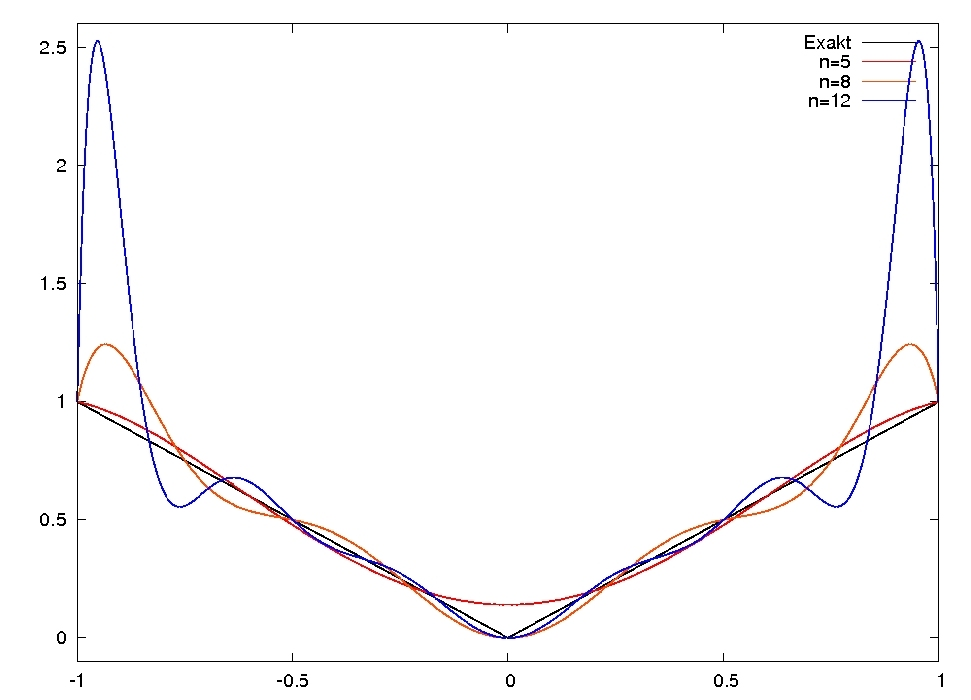
\includegraphics[width=0.5\linewidth]{images/afg49aequi.jpg}
\end{image}
\label{6.1.20im1}
\begin{image}{Gegenbeispiel zur Konvergenz: Tschebyscheff-Punkte für Betragsfunktion}
  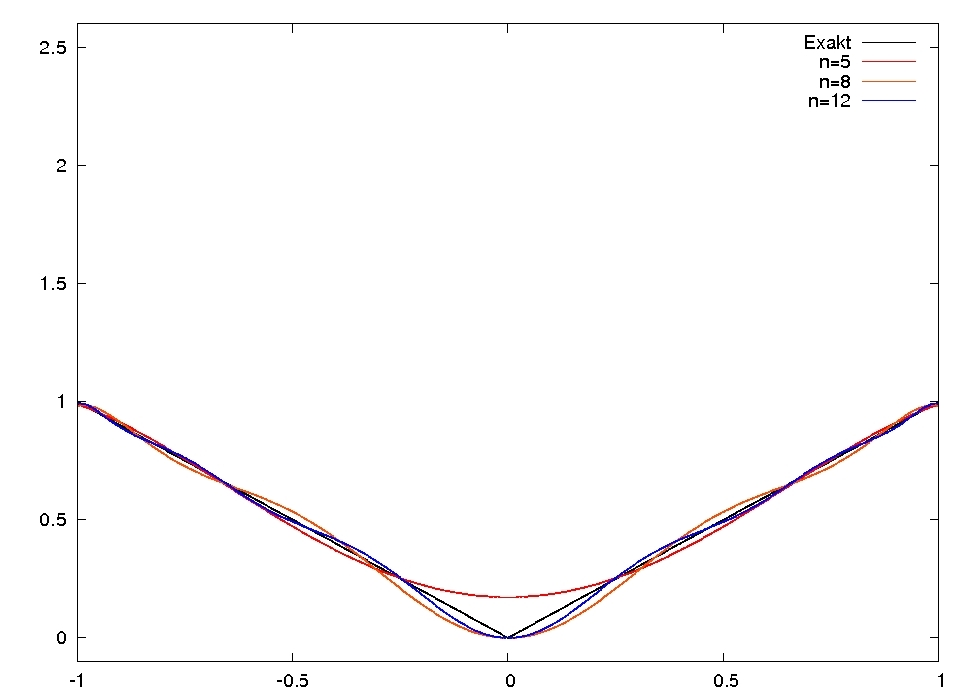
\includegraphics[width=0.5\linewidth]{images/afg49tscheby.jpeg}
\end{image}
\label{6.1.20im2}

Ein weiteres Gegenbeispiel ist $f(x)=\frac{1}{1+x^2}$ in $[-5,5]$ 
(siehe Übungsaufgabe).

Es gilt sogar:

\begin{Satze}[Faber]
  Zu jeder Folge von Intervalleinteilungen von $[a,b]$
  gibt es eine stetige Funktion $f$ ,
  so dass die Interpolationspolynome auf $[a, b]$
  nicht gleichmäßig gegen $f$ konvergiert 
  (bzgl. $\nn{\,\cdot\,}_\infty$).
\end{Satze}

Basierend auf dem Satz von Jackson gilt:
\begin{Satze}[Konvergenz bei Tschebyscheff-Knoten]
  Sei $f\in C([-1,1])$ Lipschitz-stetig.
  Dann konvergieren die Interpolationspolynome
  zu den Tschebyscheff-Knoten gleichmäßig	gegen $f$ .
\end{Satze}

Andererseits gilt \cite[siehe][]{haemmerlinhoffmann}:
\begin{Satze}[Marcinkiewicz]
  Zu jeder Funktion $f\in C([a,b])$ kann eine Folge von
  Intervalleinteilungen angegeben werden,
  so dass die Folge der Interpolationspolynome gleichmäßig gegen $f$ konvergiert.
\end{Satze}

Im Gegensatz zur $\nn{\,\cdot\,}_\infty$-Norm (auch Tschebyscheff-Norm genannt)
gilt für die $\nn{\,\cdot\,}_2$-Norm \cite[siehe][]{haemmerlinhoffmann}:
\begin{Satze}
  Sei $f\in C([-1,1])$ und seien $x_0,\dots, x_n$ die Nullstellen
  des	Legendre-Polynoms $L_n+1$. Dann gilt
  \begin{gather*}
    \lim\limits_{n\rightarrow \infty}\nn{f-p(f\mid x_0,\dots, x_n)}_2 = 0
  \end{gather*}
\end{Satze}


\sectione{Stückweise polynomiale Approximation durch Splines}
Eine hohe Anzahl von Knoten garantiert keine \enquote{gute}
Approximation durch Interpolationspolynome.
In der Regel treten dann hohe Schwingungen auf,
die unerwünscht sind.
Die Idee der stückweisen polynomialen Approximation ist,
jeweils einige wenige Stützwerte polynomial zu interpolieren
und diese \enquote{glatt} zusammenzusetzen.

\begin{image}{stückweise polynomiale Approximation}
  \begin{tikzpicture}[>=triangle 45]
    \draw[->,color=black] (0,0) -- (10,0);
    \draw[->,color=black] (0,0) -- (0,8);
    \clip(-0.5,-0.5) rectangle (10,8);
    
    \foreach \x/\text in {0.5/$a=x_0$,3.5/$x_1$,4.5/$x_2$,6/$x_3$,8.5/$x_4=b$}
    \draw (\x,0.1) -- (\x,-0.1) node[below] {\text};
    
    % k=1
    \foreach \x/\y/\wert in {0.5/3.5/4.5,3.5/4.5/1,4.5/6/1.5,6/8.5/5}
    {
      % Waagrechte Linien (chi-Funktionen)
      \draw(\x,\wert)--(\y,\wert);	
      % Beginn und Ende der Linien
      \draw(\x+0.1,\wert-0.2)--(\x,\wert-0.2)--(\x,\wert+0.2)--(\x+0.1,\wert+0.2);	
      \draw (\y-0.1,\wert-0.2) arc (-90:90:0.1 and .2);
    }
    
    % k=2 (linear)
    \foreach \x/\y/\wertx/\werty in {0.5/3.5/4.5/1,3.5/4.5/1/1.5,4.5/6/1.5/5,6/8.5/5/3.5}
    % Gerade zwischen den beiden Punkten
    \draw[color = blue] (\x,\wertx) -- (\y,\werty);
    
    \draw[color=red,smooth,samples=200,domain=0.5:6] plot(\x,{0.058*\x^3-0.073*\x^2-1.696*\x+5.359});
    \draw[color=red,smooth,samples=200,domain=6:8.55] plot(\x,{-0.293*\x^3+4.84*\x^2-24.067*\x+38.52});
  \end{tikzpicture}
\end{image}
\label{im6.2}

\begin{itemize}
\item stückweise linear und stetig ist am einfachsten
\item stückweise kubisch und global zweimal stetig differenzierbar
  ist zur graphischen Aufarbeitung am geeignetsten,
  da das Auge noch Unstetigkeiten in der Krümmung erkennt.
\end{itemize}


\extrasection{a)}{Splines und zwei verschiedene Basen}
\begin{Defe}\index{Spline}
  Sei $\Delta =\{x_0,\dots,x_n\} $ ein Gitter
  mit paarweise verschiedenen Knoten $a=x_0<\dots<x_n=b$.\\
  Ein (Polynom-)\textbf{Spline von Ordnung $k$}$\geq 2$ 
  (d.h. der Grad der Teilstückpolynome ist maximal $(k-1)$)
  ist eine Funktion $s$ mit $s\in C^{(k-2)}([a,b])$
  und $s\in\p_{k-1}([x_i,x_{i+1}])$
  für $i=0,\dots,n-1$.\\
  Der Raum der Splines von Ornung $k$ bzgl. $\Delta$ sei
  mit $S_{k,\Delta}$ bezeichnet.\\
  Für $k=1$ ist der Raum definiert durch
  \begin{gather*}
    S_{1,\Delta} \coloneqq 
    \left\{
      s:[a,b]\rightarrow\R\,\middle\vert\,
      s|_{[x_i,x_{i+1}]}\in\p_0
      \text{ für } 0\leq i\leq n
    \right\}
  \end{gather*}
  Für $k=2$ ergeben sich \textbf{lineare Splines}\index{Spline!linear}
  und für $k=4$ die \textbf{kubischen Splines}\index{Spline!kubisch}.\\
  Offensichtlich gilt
  \begin{enumerate}[a)]
  \item $S_{k,\Delta}$ ist ein linearer Vektorraum.
  \item $\p_{k-1}\subseteq S_{k,\Delta}$
  \end{enumerate}
  Natürlich lässt sich ein Spline stückweise als Polynom darstellen,
  es hat also $n\cdot k$ Koeffizienten.
  Gewünscht ist aber eine Basisdarstellung,
  welche dann $n+k-1$ Koeffizienten hat.
\end{Defe}

\begin{Satze}\label{6.2.2}\index{abgebrochene Potenz}
  Die Monome $x^l$ und die \textbf{abgebrochenen Potenzen}
  \begin{gather}
    (x-x_i)_+^l\coloneqq
    \begin{cases}
      (x-x_i)^l & x\geq x_i\\
      0         & x<x_i
    \end{cases}
    \label{VI.2.1}
  \end{gather}
  bilden eine Basis\index{Splineraumbasis}
  \begin{gather*}
    \mathcal{B}=
    \left\{
      1,x,\dots,x^{k-1},(x-x_1)+^{k-1},\dots,(x-x_{n-1})_+^{k-1}
    \right\}
  \end{gather*}
  des Splineraumes $S_{k,\Delta}$. Insbesondere gilt
  \begin{gather}
    \dim S_{k,\Delta}=k+n-1
    \label{VI.2.2}
  \end{gather}
  \imagemissing{Dimension eines Splineraumes}\label{im6.2.2}

  \begin{proof}
    siehe Übungsaufgabe
  \end{proof}
\end{Satze}


% --------------------------------------


\subsectione{Nachteile der Splineraumbasis}
\begin{enumerate}[a)]
\item Basisfunktionen haben keine lokalen Träger,
  d.h. zur Auswertung von $s(\overline{x})$ müssen
  alle Basisfunktionen ausgewertet werden, was relativ teuer ist.
\item Falls $x_i\approx x_{i+1}$ sind 
  $(x-x_i)_+^{k-1}$ und $(x-x_{i+1})_+^{k-1}$
  nahezu linear unabhängig.\\
  Damit ist die Basis schlecht konditioniert bzgl. Störungen in $b_i$.
\end{enumerate}

Das Ziel ist nun eine bessere Basis zu konstruieren.

\begin{Bspe}~
  \begin{enumerate}[a)]
  \item \index{Splineraumbasis!$S_{1,\Delta}$-Basis}
    $S_{1,\Delta}$ sind stückweise konstante Funktionen

    \begin{image}{Basis eines $S_{1,\Delta}$-Splines aus stückweise konstanten Elementen}
      \begin{tikzpicture}[>=triangle 45]
        \draw[->,color=black] (0,0) -- (10,0);
        \draw[->,color=black] (0,0) -- (0,5);
        \clip(-0.5,-0.5) rectangle (10,5);
        
        \foreach \x/\text in {0.5/$x_0$,3.5/$x_1$,4.5/$x_2$,6/$x_3$,8.5/$x_4$}
        \draw (\x,0.1) -- (\x,-0.1) node[below] {\text};
        
        % k=1
        \foreach \x/\y/\wert in {0.5/3.5/3.5,3.5/4.5/1,4.5/6/1.5}
        {
          % Waagrechte Linien (chi-Funktionen)
          \draw(\x,\wert)--(\y,\wert);	
          % Beginn und Ende der Linien
          \draw(\x+0.1,\wert-0.2)--(\x,\wert-0.2)--(\x,\wert+0.2)--(\x+0.1,\wert+0.2);	
          \draw (\y-0.1,\wert-0.2) arc (-90:90:0.1 and .2);
        }
        
        \draw (6,4)--(8.5,4);
        \draw(6+0.1,4-0.2)--(6,4-0.2)--(6,4+0.2)--(6+0.1,4+0.2);
        \draw(8.5-0.1,4-0.2)--(8.5,4-0.2)--(8.5,4+0.2)--(8.5-0.1,4+0.2);
      \end{tikzpicture}
    \end{image}
    \label{im6.2.4(1)}

    Die zugehörige Basis wie oben beschrieben wäre
    \begin{gather*}
      \left\{ 1,(x-x_i)_+^0\right\}
    \end{gather*}
    Eine in diesem Fall geeignetere Basis ist
    \begin{gather*}
      N_{i,1} (x)\coloneqq \chi_{[x_{i-1},x_i)}(x)
      = \begin{cases}
        1 & \text{falls } x\in[x_{i-1},x_i)\\
        0 & \text{sonst}
      \end{cases}\, ,
    \end{gather*}
    womit die Darstellung eines $S_{1,\Delta}$-Splines zu 
    \begin{gather*}
      s(x) = \sum_{j=1}^{n+1} f_{j-1} N_{j,1}(x)
    \end{gather*}
    wird.
  \item \index{Splineraumbasis!$S_{2,\Delta}$-Basis} $S_{2,\Delta}$ sind stückweise lineare, global stetige
    Funktionen. Eine Basis wie in \ref{6.2.2} ist
    \begin{gather*}
      \left\{1,x^1, (x-x_i)_+^1\right\}
    \end{gather*}
    \imagemissing{Basis eines $S_{2,\Delta}$-Splines mit Hutfunktion (siehe auch \ref{6.2.6} für allg. Hutfunktionen)}\label{im6.2.4(2)}
    Hier kann eine Basis wie oben durch sog. 
    \textbf{Hutfunktionen}\index{Hutfunktion}
    konstruiert werden
    \begin{align*}
      N_{i,2}(x_{j-1}) &= \delta_{i,j}\\
      N_{i,2}(x) &= \begin{cases}
        ~\frac{1}{x_{i-1}-x_{i-2}}(x-x_{i-2}) & x\in [x_{i-2}, x_{i-1}]\\
        -\frac{1}{x_{i-1}-x_{i-2}}(x-x_{i-1})+1 & x\in [x_{i-1}, x_i]
      \end{cases}
    \end{align*}
    \imagemissing{allgemeine Hutfunktion am Punkt $x_i$ eines $S_{2,\Delta}$-Splines}\label{im6.2.4(3)}
    Ein Spline, welches $f$ in $x_i$ interpoliert hat dann die Form
    \begin{gather*}
      s(x) = \sum_{j=1}^{n+1}f_{j-1}N_{j,2}(x)
    \end{gather*}
  \end{enumerate}
\end{Bspe}


\begin{Defe}
  Sei $t_1\leq \dots \leq t_m$ eine beliebige Folge von Knoten
  $x_i$.\\
  Dann sind die \textbf{B-Splines}\index{Spline!B-Splines}
  $N_{j,l}$ für $l=1,\dots, m$ und $j=1,\dots, m-l$ 
  rekursiv erklärt durch
  \begin{align}\nonumber
    N_{j,1}(x) &\coloneqq \chi_{[t_j,t_{j+1})}(x) 
                 \text{ für } t_{j+1}\neq t_j\\
    N_{p,1}(x) &= \chi_{[t_p,t_m]}(x) 
                 \text{ für }
                 p=\min\left\{i\,\middle\vert\,t_{i+1}=t_m\right\}
                 \label{VI.2.3}
  \end{align}
  sowie für $l>1$
  \begin{gather}
    N_{j,l} (x) = \frac{x-t_j}{t_{j+l-1}-t_j}N_{j,l-1}(x) 
    +  \frac{t_{j+l}-x}{t_{j+l}-t_{j+1}}N_{j+1,l-1}(x) 
    \label{VI.2.4}
  \end{gather}
  Hierbei gilt die Konvention $\frac{0}{0}=0$, 
  denn für $t_j=t_{j+l-1}$ gilt
  $N_{j,1}\equiv 0$ und auch $N_{j,l-1}\equiv 0$.
\end{Defe}


Ziel ist nun u.a. mit diesem eine Basis von $S_{k,\Delta}$ anzugeben,
die zudem gut konditioniert ist.
Vorher jedoch werden noch einige Eigenschaften der B-Splines
untersucht.


\subsectione{Gestalt der B-Splines}\label{6.2.6}
Bei einem B-Spline $N_{j,k}$ entspricht $j$ dem Ort und
$k-1$ entspricht dem Polynomgrad.

\begin{image}{}
  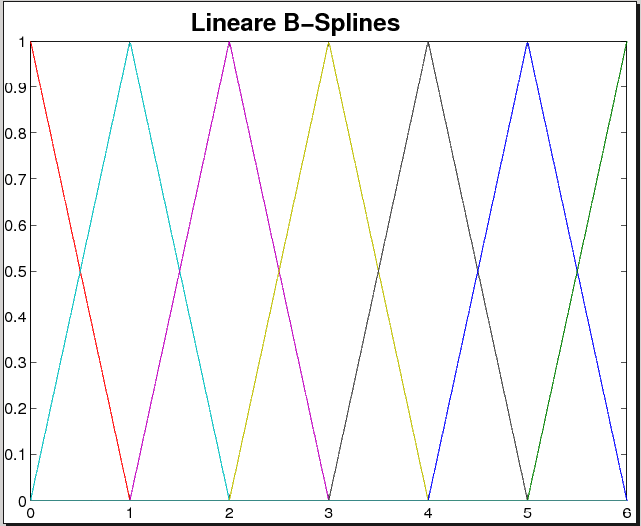
\includegraphics[width=\linewidth]{images/linBsplines.png}
\end{image}
\begin{image}{}
  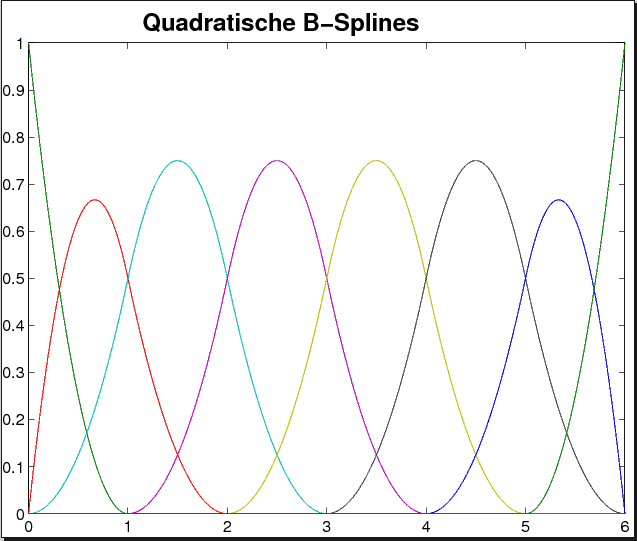
\includegraphics[width=\linewidth]{images/quadBsplines.png}
\end{image}
\begin{image}{}
  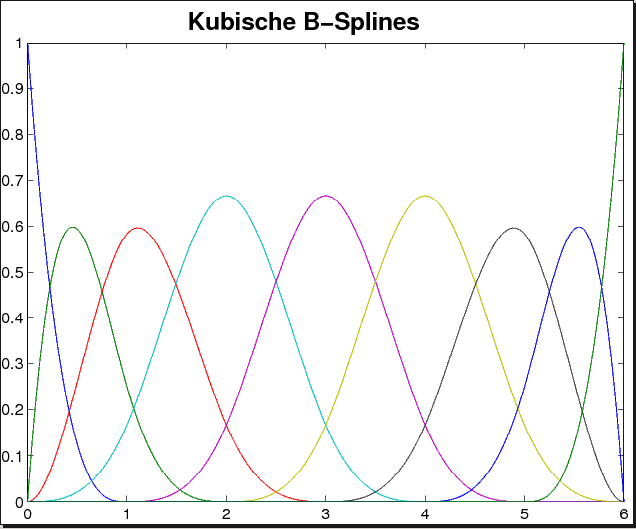
\includegraphics[width=\linewidth]{images/kubBsplines.png}
\end{image}

\begin{Kore}
  Es gilt
  \begin{enumerate}[a)]
  \item $supp N_{j,k} \coloneqq 
    \overline{\left\{ x\in[a,b]\,\middle\vert
        \, N_{j,k}(x)\neq 0\right\}} \subset [t_j, t_{j+1}]$
    (lokaler Träger)
  \item $N_{j,k}>0 ~\forall x\in(t_j,t_{j+1})$ (nicht negativ)
  \item $N_{j,k}\vert_{[t_l,t_{l+1})}\in \p_{k-1}$
  \end{enumerate}

  \begin{proof}
    siehe Übungsaufgabe
  \end{proof}
\end{Kore}

\subsectione{Auswertung von $s$ an der Stelle $\overline{x}$}
\label{6.2.8}
Sei $\overline{x}\in[t_j,t_{j+1}]$ und
$s(x) = \sum_{i=1}^{N}c_iN_{i,k}(x)$.
Da nur $N_{j,1}(\overline{x})\neq 0$ ist, 
können aufgrund von \eqref{VI.2.4}
auch nur $N_{j-k+1, k}(\overline{x}), \dots, N_{j,k}(\overline{x})$
verschieden von Null sein, da
\begin{align*}
  \begin{array}{ccccccccc}
    j\backslash l & t_j & 1 && 2 && 3 &&k\\
    \cline{1-9}
    1 & t_1 & N_{1,1}(\overline{x})=0 &&0&&0&&0\\
                  &&0&&\vdots&&\vdots&&\vdots\\
                  &&\vdots &&&&&&0\\
    j-k+1&t_{j-k+1} &\dots &&\dots&&\dots&&\boldsymbol{N_{j-k+1,k}(\overline{x})} \\
    \vdots&\vdots&&&&&&&\vdots\\
                  && &&0&& \boldsymbol{N_{j-2,3}(\overline{x})}
                                 &&N_{j-2,k}(\overline{x})\\
    j-1 & t_{j-1} &0 &\longrightarrow & \boldsymbol{N_{j-1,2}(\overline{x})}
                                      &\longrightarrow & N_{j-1,3}(\overline{x})
            && N_{j-1,k}(\overline{x})\\
    j& t_j & \boldsymbol{N_{j,1}(\overline{x})=1}&\longrightarrow&\boldsymbol{N_{j,2}(\overline{x})}
                                      &\longrightarrow&\boldsymbol{N_{j,3}(\overline{x})}&\longrightarrow\dots&\boldsymbol{N_{j,k}(\overline{x})}\\
                  &&0&&0&&&&\vdots\\
                  &&\vdots &&\vdots\\
                  &t_{j+k}&0&&0&&&&0
  \end{array}
\end{align*}

Daraus folgt, dass $N_{i,k}(\overline{x})\neq x$ 
für höchstens $i=j-k+1,\dots, j$.\\
Nach der Rekursionsformel baut $N_{i,k}$ auf 
$N_{i,1},\dots , N_{i+(k-1),1}$ auf und
benutzt $t_i,\dots, t_{i+k}$.\\
Da in der Rekursionsformel nur nichtnegative Vielfache
nichtnegativer Zahlen addiert werden,
ist das Verfahren zur Bestimmung der $N_{i,k}(\overline{x})$
numerisch sehr stabil.

\begin{Leme}
  Falls $t_j<t_{j+k}$ und $x\neq t_m$,
  so gilt
  \begin{gather}
    N_{j,k}(\overline{x})=(t_{j+k}-t_j)\underset{
      [t_j,\dots, t_{j+k}]f\text{ mit } f(t)\coloneqq (t-x)_+^{k-1}}
    {[t_j,\dots,t_{j+k}](\bullet -x)_+^{k-1}}
    \label{VI.2.5}
  \end{gather}
\end{Leme}

\begin{proof}
  kein Beweis.

  Idee: Per Induktion über $k$. Nutze hierfür
  \begin{gather*}
    (t-x)_{+}^k = (t-x)(t-x)_{+}^{k-1}\,,\, k \geq 1,
  \end{gather*}
  sowie $[t_j , \dotsc, t_i]( \bullet - x) = 0$ für $i > j+1$ und die Leibnizregel.
\end{proof}

Zu gegebenem Splineraum $S_{j,\Delta}$ mit
% Nummerierung
\begin{gather}
  \Delta a=x_0 < x_1 < \dotsm < x_n = b
  \label{VI.2.6}
\end{gather}
Setzt man nun 
\begin{gather}
  T: t_1 = \dotsm = t_k < t_{k+1} < \dotsm < t_{k+n} =
  t_{n+2k+1}\, ,
  \label{VI.2.7}
\end{gather} lässt sich folgender Satz zeigen:


% --------------------------------


\begin{Satze}\label{6.2.10}~
  \marginpar{17.12.2014}
  \begin{enumerate}
  \item Es gilt 
    $\p_{k-1}\subset
    span\left\{N_{1,k}, \dots, N_{n+k-1,k}\right\}$
  \item Die B-Splines bilden eine Zerlegung der Eins auf $[a,b]$,
    d.h. 
    \begin{gather*}
      1\equiv \sum_{j=1}^{n+k-1}N_{j,k}(x) \quad \forall x\in[a,b]
    \end{gather*}
  \item Weiterhin sind die B-Splines (lokal) linear unabhängig,
    d.h. falls
    \begin{gather*}
      \sum_{l=1}^{n+k-1}c_lN_{l,k}(x)=0 
      \quad\forall x\in(c,d)\subset [a,b]\,,
    \end{gather*}
    folgt $c_j=0$ für alle $j$ mit 
    $(c,d)\cap \underbrace{(t_j,t_j+k)}_{=supp N_{j,k}}\neq \varnothing$.
    \imagemissing{Lineare Unabhängigkeit der B-Splines}\label{im6.2.10}
  \end{enumerate}

  \begin{proof}~
    \begin{description}
    \item[a), b)] folgen aus der Marschen-Identität 
      \cite[siehe z.B.][]{deuflhardhohmann}
    \item[c)] O.B.d.A. enthalte $(c,d)$ keine Knoten $t_i$
      (sonst zerlege $(c,d)$ in Teilintervalle).
      Dann folgt $(c,d)\subseteq (t_l, t_{l+1})$.
      Nach a) lässt sich jedes Polynom $p\in \p_{k-1}$
      durch die B-Splines $N_{l,k}$ darstellen.
      Auf $(c,d)$ sind nur $k=dim\p_{k-1}$
      B-Splines von Null verschieden.
      Daher müssen diese linear unabhängig sein.
    \end{description}
  \end{proof}
\end{Satze}

\begin{Fole}
  Die B-Splines $\{N_{1,k},\ldots,N_{n+k-1,k}\}$ bilden eine Basis von 
  $S_{k,\Delta}$.

  Die Koeffizienten $c_i$ der Basisdarstellung von $s \in S_{k,\Delta}$
  \begin{gather*}
    s(x)=\sum_{i=1}^{n+k-1}c_iN_{ik}(x)
  \end{gather*}
  heißen \textbf{de Boor-Punkte}\index{de Boor-Punkte} von $s$. \\
  Die Funktionswerte $s(x)$ sind somit eine
  Konvexkombination der de Boor-Punkte $c_i$.
\end{Fole}


\begin{Beme}
  Die B-Spline Basis ist eine gut konditionierte Basis, d.h.
  die Auswertung von Splines mittels ihrer B-Spline
  Darstellung ist gut konditioniert.
  Es gilt mit $N\coloneqq n+k-1$
  \begin{gather*}
    D_k \max_{j=1,\ldots, N} |c_j| 
    \leq \nn{\sum^N_{j=1} c_j N_{jk}}_{\infty}
    \leq \max_{j=1,\ldots, N} | c_j|
  \end{gather*}
  Die Konstante $D_k$ hängt nur von der Ordnung $k$ ab, nicht
  von der Lage der Knoten.
\end{Beme}

\extrasection{b)}{Splineinterpolation}

\subsectione{Splineinterpolation allgemein}\label{6.2.13}
Gegeben seien $N=n+k-1=dimS_{k,\Delta}$ Stützpunkte $(\xi_i,f_i)$
mit
\begin{gather*}
  \xi_1<\dots<\xi_N\,.
\end{gather*}
Gesucht sind nun Splines $s\in S_{k,\Delta}$ 
mit $s(\xi_i)=f_i$ für alle $i=1, \dots, N$.
Das ist äquivalent zu 
\begin{align}
  \sum_{j=1}^N c_jN_{j,k}(\xi_i)&=f_i &&\text{für }i=1,\dots, N
                                         \label{VI.2.8}
  \\\nonumber
  \Leftrightarrow Ac&=f &&\text{mit } A=(N_{j,k}(\xi_i))_{i,j=1,\dots,N}
\end{align}

\subsectione{Lineare B-Splines}\label{6.2.14}
Sei $k=2$, $N=n+1$, $S_{2,\Delta}$ der Splineraum zu einem $\Delta$,
welches konstruiert werden soll.
\imagemissing{Stützstellen für eine konstruierte Zerlegung $\Delta$}\label{im6.2.14}
Sei $x_0\coloneqq \xi_1<x_1\coloneqq \xi_2<\dots<x_n\coloneqq
\xi_{n+1}$, dann folgt
\begin{gather*}
  N_{i,2}(\xi_j)=N_{i,2}(t_{j+1})=\delta_{i,j}
\end{gather*}
Also ist in diesem Fall die Matrix $A=(N_{j,k}(\xi_i))_{i,j\leq n}=I$
also $c_i=f_i=f(\xi_i)=f(x_{i-1})$.
Der zugehörige Spline $s$ hat dann die Form
\begin{align*}
  s(x) &= \sum_{i=1}^{N}f_i N_{i,2}(x) \\
       &= \sum_{j=0}^{N}f(x_j)N_{j+1,2}(x)
\end{align*}
Zur Auswertung von $s$ wird \ref{6.2.8} verwendet.
$A$ sei definiert als
\begin{gather*}
  A \coloneqq \left(N_{j,k}(\xi_i)\right)_{i,j=1,\ldots,N}
\end{gather*}
und hat folgende Eigenschaften
\begin{itemize}
\item  $A$ besitzt Bandstruktur, da  $\xi_i$ höchstens in $k$
  Intervallen $[t_j, t_{j+k}]$ liegen kann.
\item $A$ ist regulär, also $N_{ik}(\xi_i)\neq 0$
  für $i=1, \ldots, N$.\\
  (nach dem Satz von Schoenberg und Whitney, 1953)
\item $A$ ist total positiv, d.h. für alle quadratischen
  Untermatrizen $B$ gilt $\det(B)\geq 0$.\\    
  (nach Karlin, 1968)
\end{itemize}

Daraus kann man folgern, dass
die Gaußelimination für Bandmatrizen ohne Pivotsuche
durchführbar ist, falls $N_{ik}(\xi_i) \neq 0$
für $i =1, \ldots, N$.\\


\subsectione{Kubische B-Spline-Interpolation} \label{6.2.15}
Sei $k=4$ und entsprechend $N=n+3$ und 
seien die Stützpunkte zur Interpolation wie in \ref{6.2.14}
gegeben durch 
\begin{gather*}
  \xi_i = x_{i-1} \quad \text{ für } i=1, \ldots, n+1\,.
\end{gather*}
(Daraus folgt $N\neq n+3$ und \ref{6.2.13} ist nicht anwendbar.)\\
Zur eindeutigen Bestimmung von $s\in S_{4,\Delta}$ fehlen zwei
Bedingungen.\\
Typischerweise werden 
zusätzlich zu 
\begin{gather*}
  s(x_i)=f(x_i) \quad \text{für } i=0,\ldots,n
\end{gather*} 
eine der folgenden Randbedingungen gefordert:
\begin{enumerate}[i)]
\item $s'(a)=f'(a)$ und $s'(b)=f'(b)$:  \\
  \textbf{vollständige} oder \textbf{Hermitesche kubische 
    Spline-Interpolation} 
\item $s''(a)=s''(b)=0$ (\enquote{natürliche}  Endbedingungen):\\
  \textbf{natürliche kubische Spline-Interpolation}\\
  (d.h. $s$ kann linear außerhalb von $[a,b]$ glatt fortgesetzt
  werden) 
\item $s'(a)=s'(b)$ und $s''(a)=s''(b)$,
  falls $f$ periodisch mit Periode $b-a$ ist: \\
  \textbf{periodische kubische Spline-Interpolation}.
\end{enumerate}
Die drei Randbedingungen werden aufgrund physikalischer
Eigenschaften gefordert. Hierzu ein Beispiel: 

Es beschreibe $y(t)$ die Lage eines
homogenen, isotropen Stabes (z.B. eine dünne Holzlatte).
Dann misst
\begin{gather*}
  E(y) = c \int_a^b\left(
    \frac{y''(t)}{(1+y'(t)^2)^{\frac{3}{2}}}
  \right)^2dt
  = c \int_a^b\left(
    \kappa(t)
  \right)^2dt
\end{gather*}
(wobei $\kappa $ die Krümmung der Kurve $y$ in der Ebene ist) 
die Biegeenergie.\\
Aufgrund des \textbf{Hamiltonschen Prinzips}\index{Hamiltonsches Prinzip}
stellt sich der Stab so ein, dass $E(y)$ minimiert wird.\\
Unter der Annahme $|y'(t)| \ll 1$ für $t\in [a,b]$ 
wird $E$ linearisiert zu $c\int_a^by''(t)^2dt$.
Also wird annähernd eine Funktion $y\in C^2$ gesucht,
welche $\nn{y''}_2^2$ minimiert.

Obige Splines haben gerade diese Eigenschaft, denn:

\begin{Satze}\label{6.2.16}
  Sei $s$ ein interpolierender, kubischer Spline von $f$
  in den Knoten $x_i $ und $y\in C^2$ eine beliebige Funktion
  von $f$, so dass 
  \begin{gather*}
    \left[s''(t)\cdot(y'(t)-s'(t))\right]_{t=a}^{b}=0
  \end{gather*}
  Dann gilt $\nn{s''}_2 \leq \nn{y''}_2$.

  \begin{proof}
    Es gilt
    \begin{align*}
      \nn{y''}_2^2 &= \nn{s''+(y''-s'')}_2^2\\
                   &= \nn{s''}_2^2
                     + 2\underbrace{\int_{a}{b}s''(y''-x'')dt}_{
                     \mathclap{\substack{=0 \\ \text{ wie gezeigt wird}}}
      }
      + \nn{y''-s''}_2^2
    \end{align*}
    da
    \begin{align*}
      \int_{a}^{b} s''(y''-x'')dt &= \sum_{i=1}^{N}\left(\left[
                                    s''(y'-s')\right]_{x_{i-1}}^{x_i}
                                    -\int_{x_{i-1}}^{x_i}s'''(y'-s')dt\right)\\
      \intertext{($S_{4,\Delta}\subseteq C^2([a,b])$, 
      $s'''(x)\equiv d_{i-1}=const$, 
      da 
      $s\in\p_3([x_{i-1},x_i])$ )
      }
                                  &= \underbrace{\left[ s''(y'-s')\right]_{a}^{b}}_{
                                    \mathclap{\substack{ =0 \\ \text{ nach Voraussetzung } }}
      }
      -\sum_{i=1}^{N} d_{i-1}
      \int_{x_{i-1}}^{x_i} \left(y'(t)-s'(t)\right) dt\\
                                  &=-\sum_{i=1}^N d_{i-1}\bigg(\big(y(x_i)-s(x_i)\big)
                                    - \big(y(x_{i-1})-s(x_{i-1})\big)\bigg) \\
                                  &=0
    \end{align*}
    da $y$,$s$ Interpolationen von $f$ sind.\\
    Mit den Randbedingungen i), ii) und iii) 
    ist die Voraussetzung von \ref{6.2.16} erfüllt.
  \end{proof}
\end{Satze}

\begin{Kore}\label{6.2.17}
  Es existiert genau ein interpolierender kubischer Spline 
  $s\in S_{4,\Delta}$, welcher die Randbedingungen aus \ref{6.2.16}
  erfüllt.
  Weiterhin gilt für jede interpolierende Funktion $y\in C^2([a,b])$,
  die derselben Randbedingung genügt
  \begin{gather*}
    \nn{s''}_2 \leq \nn{y''}_2
  \end{gather*}

  \begin{proof}
    Die Anzahl der Forderungen ist $N=dim S_{4,\Delta}$.
    Es ergibt sich also ein quadradratisches lineares Gleichungssystem
    und es genügt Injektivität zu zeigen.\\
    Sei $f\equiv 0$, dann erfüllt $y\equiv 0$ alle Forderungen.
    für alle Lösungen $s\in S_{4,\Delta}$ gilt daher
    \begin{gather*}
      \nn{s''}_2\leq \nn{y''}_2 =0 \quad \text{ nach \ref{6.2.16}}
    \end{gather*}
    Also gilt $s''\equiv 0$ und $s$ ist stückweise kubische Funktion
    mit $s\in C^2([a,b])$  und $s(x_i)=0$.
    Damit folgt $s\equiv 0$, was die Injektivität zeigt.
  \end{proof}
\end{Kore}

% ----------------------------------------------------


\subsectione{Berechnung der natürlichen Splines mittels B-Splines}
\label{5.2.18}
\marginpar{22.12.2014}
\begin{gather*}
  A \coloneqq 
  \left(\begin{array}{ccccccccc}
          \frac{x_2+x_1-2x_0}{x_2-x_0}& & -\frac{x_1-x_0}{x_2-x_0}& && & & & \\
          N_{2,4}(x_1)&&N_{3,4}(x_1) &&N_{4,4}(x_1)  & &&&0 \\
                                      &\ddots & &\ddots& &\ddots &  &&\\
                                      & & N_{i+1,4}(x_i)&& N_{i+2,4}(x_i) && N_{i+3,4}(x_i) && \\
                                      & &  &\ddots& &\ddots &&\ddots  &\\
          0&&&  &N_{n,4}(x_{n-1}) &&N_{n+1,4}(x_{n-1}) &&N_{n+2,4}(x_{n-1}) \\
                                      & & && && -\frac{x_n-x_{n-1}}{x_n-x_{n-2}} && \frac{2
                                                                                    x_n-x_{n-2}-x_{n-1}}{x_n-x_{n-2}}
        \end{array}\right)
    \end{gather*}
    Die Werte $N_{j,4}(x_i)$ lassen sich nach \ref{6.2.8} berechnen.


    Insbesondere ergibt sich für äquidistantes Gitter
    \begin{equation*}
      \frac{1}{12}
      \left(\begin{array}{ccccccc}
              18& -6&&&&&\\
              3&7&2&  &&&\\
                &2&8&2  &&&\\
                & &\ddots &\ddots &\ddots &&\\
                & & & 2&8&2&\\
                & & & &2&7&3\\
                & & &&&-6&18\\
            \end{array}\right) 
          \left(\begin{array}{c}
                  c_2\\ \\ \vdots \\ \\c_{n+2}
                \end{array}\right)
              =
              \left(\begin{array}{c}
                      f_0\\ \\ \vdots \\ \\f_n
                    \end{array}\right)
                \end{equation*}
                (siehe Übung).


                \begin{Bspe}[Laster]\label{5.2.20}
                  Das folgende Beispiel zeigt,
                  dass sowohl die Glattheit der Funktion
                  wie auch die Knotenverteilung einen Einfluß hat,
                  da die zugehörige Funktion nicht differenzierbar ist,
                  bzw. die Ableitungen betragsmäßig sehr groß sind.

                  Natürliche Spline-Interpolation
                  versus polynomiale Interpolation:\\
                  \begin{image}{Splines versus Polynominterpolation}
                    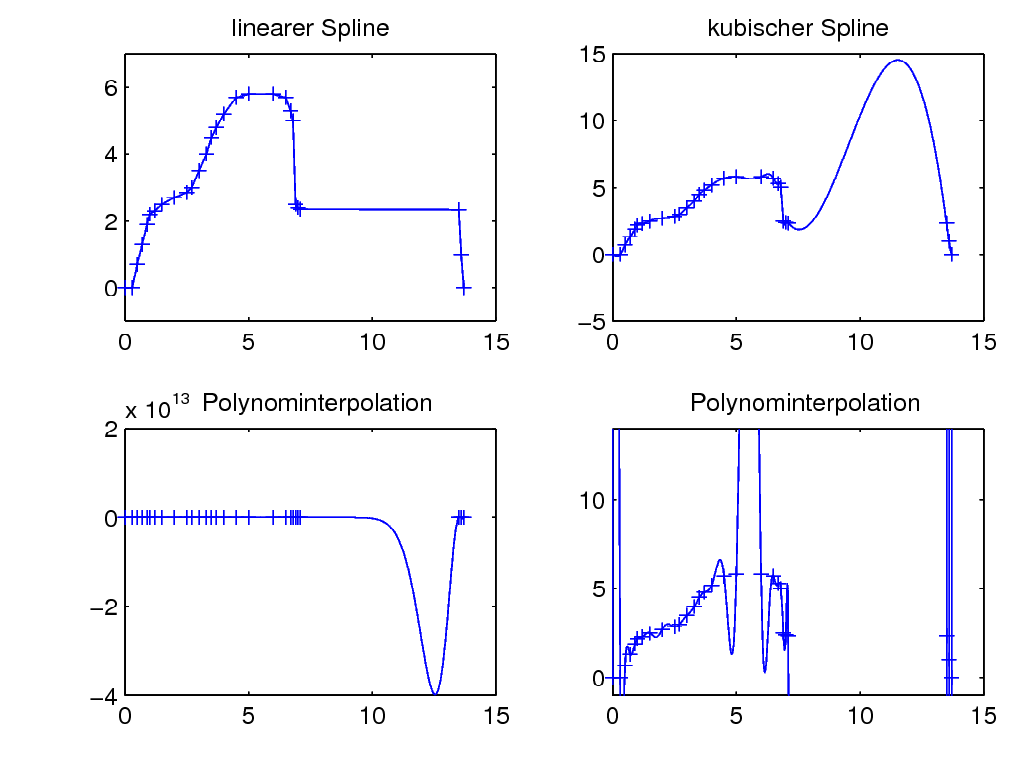
\includegraphics[width=\linewidth]{images/laster1.png}
                  \end{image}

                  Mit mehr Stützstellen:\\
                  \begin{image}{Splines versus Polynominterpolation
                      mit vielen Stützstellen}
                    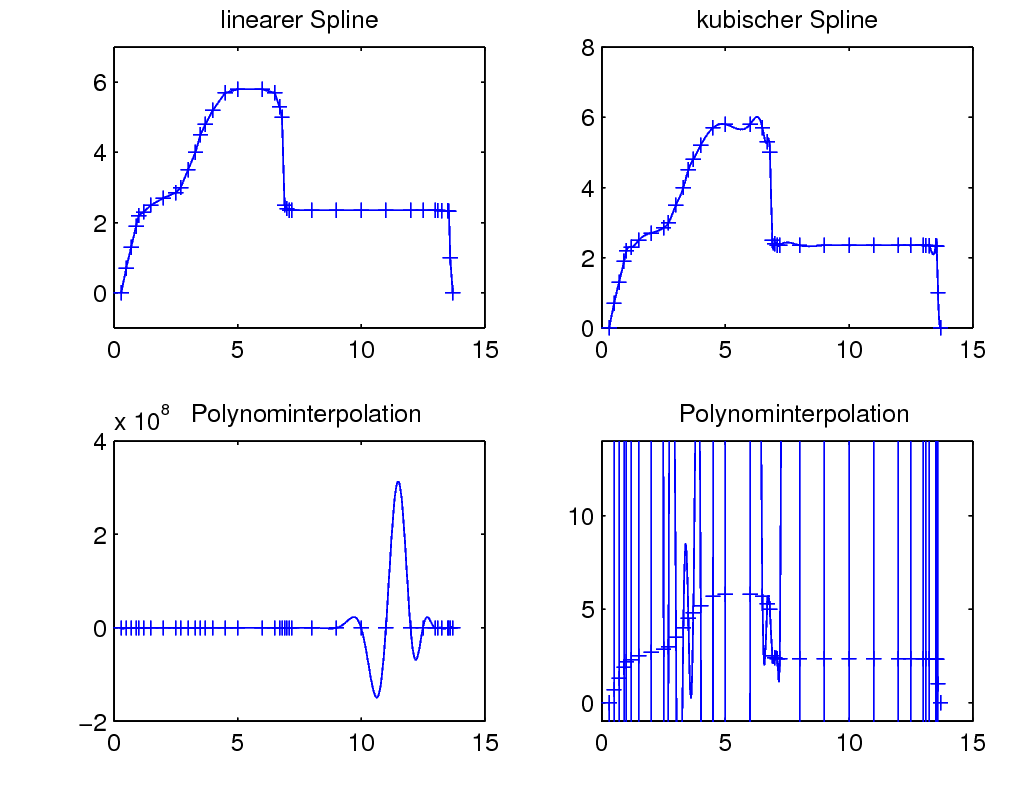
\includegraphics[width=\linewidth]{images/laster2.png} 
                  \end{image}
                \end{Bspe}

                \begin{Satze}[Fehlerabschätzung für kubische Splines]\label{5.2.21}
                  Sei $f\in C^4([a,b])$ und $s\in S_{4,\Delta}$ 
                  der interpolierende, vollständige, kubische Spline 
                  zu äquidistanten Knoten mit $h=x_{i+1}-x_i$. Dann gilt
                  für $k=0,1,2,3$
                  \begin{gather*}
                    \nn{f^{(k)}-s^{(k)}}_{\infty}\leq c_kh^{4-k}\nn{f^{(4)}}_{\infty}
                  \end{gather*}
                  mit $c_0=\frac{5}{384}$, $c_1=\frac{1}{24}$, $c_2=\frac{3}{8}$,
                  $c_3=1$, wobei $c_0$ und $c_1$ optimal sind.

                  \begin{proof}
                    \cite[siehe z.B.]
                    [(in allgemeiner Form, d.h. auch für nicht gleichmäßiges Gitter)]
                    {stoerbulirsch}\\
                    Die optimalen $c_k$ wurden von Hall und Meyer (1976) bewiesen.
                    Oft wird mit Stetigkeitsmodulen gearbeitet.
                  \end{proof}
                \end{Satze}


                Für eine wachsende Anzahl der Knoten ergibt sich also Konvergenz,
                anders als bei polynomialer Interpolation.


                \begin{Satze}[Fehlerabschätzung für lineare Splines]\label{6.2.22}
                  Sei $f\in C^2([a,b])$ und $s\in S_{2,\Delta}$
                  der interpolierende Spline  an den Stützstellen 
                  $a=x_0<x_1<\ldots<x_n=b$. 
                  Dann gilt mit $h=max_{i=0,\ldots,n-1}|x_{i+1}-x_i|$
                  \begin{gather*}
                    \nn{f-s}_{\infty}\leq \frac{h^2}{8}\nn{f''}_{\infty} \, .
                  \end{gather*}

                  \begin{proof} 
                    siehe Übungsaufgabe
                  \end{proof}
                \end{Satze}


                Weitere Literatur zu
                Splines: \cite{boor}

                %%% Local Variables:
                %%% mode: latex
                %%% TeX-master: "../numerik_script"
                %%% End:
